%%
%% Commands for TeXCount
%TC:macro \cite [option:text,text]
%TC:macro \citep [option:text,text]
%TC:macro \citet [option:text,text]
%TC:envir table 0 1
%TC:envir table* 0 1
%TC:envir tabular [ignore] word
%TC:envir displaymath 0 word
%TC:envir math 0 word
%TC:envir comment 0 0

%%
%% For anonymous submission (double-blind review), use:
\PassOptionsToPackage{table}{xcolor}
\documentclass[sigconf,anonymous,review,9pt]{acmart}

%%
\AtBeginDocument{%
  \providecommand\BibTeX{{%
    Bib\TeX}}}

%%
\setcopyright{acmlicensed}
\copyrightyear{2026}
\acmYear{2026}
\acmDOI{XXXXXXX.XXXXXXX}
\acmConference[ICCAD'26]{IEEE/ACM International Conference on Computer-Aided Design}{November 8 to 12, 2026}{San Jose, CA, USA}
\acmISBN{978-1-4503-XXXX-X/26/11}

%%
\usepackage{amsmath,amsfonts}
\usepackage{multirow}
\usepackage{algorithm}
\usepackage{algorithmic}
\usepackage{booktabs}
\usepackage{subcaption}
\usepackage{url}
\definecolor{posstrong}{HTML}{C6EFCE}   % green – strong positive rho
\definecolor{posweak}{HTML}{E2EFDA}     % light green – moderate positive
\definecolor{neutral}{HTML}{F2F2F2}     % grey – near-zero rho
\definecolor{negweak}{HTML}{FDE8E8}     % pink – negative rho
\definecolor{rankfirst}{HTML}{FFCCCC}   % light red – best
\definecolor{ranksecond}{HTML}{CCE5FF}  % light blue – second best

\usepackage{caption}
\captionsetup{font=small}

\newcommand{\tpm}{$\pm$}

\begin{document}

\title{PPAPlace: Differentiable Cross-Stage Objectives for Chip Placement Optimization}

\author{Ruogu Chen}
\affiliation{%
  \institution{University of Alberta}
  \department{Department of Electrical and Computer Engineering}
  \city{Edmonton}
  \state{AB}
  \country{Canada}
}
\email{ruogu@ualberta.ca}

\author{Jie Han}
\affiliation{%
  \institution{University of Alberta}
  \department{Department of Electrical and Computer Engineering}
  \city{Edmonton}
  \state{AB}
  \country{Canada}
}
\email{jhan8@ualberta.ca}

%% ============================================================
\begin{abstract}
Chip placement is usually optimized with fast proxies such as
half-perimeter wirelength (HPWL) and pre route timing estimates, yet
these proxies often fail to rank placements by final post route timing.
This paper first studies which design flow stage provides supervision
that preserves final timing order. Across ten ChiPBench circuits and
twenty controlled placement configurations per circuit, HPWL and pre
route timing show near zero rank correlation with post detailed route
worst negative slack (WNS) and total negative slack (TNS), while post
global routing (GRT) gives consistently high fidelity at a fraction of
the full route cost. Based on this finding, we propose PPAPlace, a
differentiable timing surrogate over the full mixed size placement
state. The surrogate combines graph attention over netlist connectivity
with spatial convolution over density, pin, macro, and congestion
features. Since the feature extraction and predictor are differentiable,
predicted timing gradients can flow back to cell coordinates. PPAPlace
uses these gradients in two deployment modes. CoOpt injects the
surrogate into DREAMPlace as a learned timing objective after warmup.
Refine applies projected gradient descent to improve a completed
placement. On held out ChiPBench circuits stratified by design lineage,
PPAPlace reduces post route WNS by [AVG_WNS_IMP]\% and TNS by
[AVG_TNS_IMP]\% on average, with [GROUP_B_WNS_IMP]\% WNS and
[GROUP_B_TNS_IMP]\% TNS reduction on unseen family Ariane designs.
On out of domain designs, it reduces WNS by [GROUP_C_WNS_IMP]\% and
TNS by [GROUP_C_TNS_IMP]\%. Power remains within [POWER_RANGE]\%,
routed wirelength remains within [RWL_RANGE]\%, and all reported
placements have [DRC_COUNT] design rule violations. Code is available at
\url{https://anonymous.4open.science/r/PPAPlace}.
\end{abstract}

\keywords{chip placement, timing optimization, cross-stage prediction, differentiable objectives, graph attention network, physical design}

\maketitle

%% ============================================================
\section{Introduction}
\label{sec:intro}

Chip placement determines the physical locations of circuit modules and
standard cells. It also determines whether the routed design can meet
timing. Modern placers therefore need objectives that are cheap enough
to optimize during placement and faithful enough to predict final
post route behavior.

Most placement methods still optimize half-perimeter wirelength
(HPWL) and density. Analytical placers such as
DREAMPlace~\cite{lin2019dreamplace} optimize smooth approximations of
these objectives with GPU accelerated gradient descent. AI based
placers use reinforcement learning~\cite{mirhoseini2021graph,
lai2022maskplace, lai2023chipformer}, black box
optimization~\cite{shi2023wire}, or diffusion
models~\cite{lee2024chip}. The optimization methods differ, but the
training or search signal is usually still HPWL or another fast
pre route proxy.

The difficulty is that these proxies do not reliably rank placements by
final timing. ChiPBench~\cite{chipbench2025} evaluates AI based placers
through the full OpenROAD~\cite{ajayi2019openroad} flow and reports a
Pearson correlation of only $-0.08$ between macro HPWL and WNS. The same
benchmark shows that wirelength optimized AI placers can degrade final
timing relative to Hier-RTLMP, OpenROAD's hierarchy aware macro placer.
This result suggests that better optimization alone is not enough when
the optimized signal is weakly coupled to post route timing.

Cross stage prediction is a natural response. A learned model can score
placement candidates using labels from a later stage of the design flow.
However, such a model is only useful if its training labels preserve the
rank order of final routed timing. If the label stage reverses or
scrambles that order, a more expressive predictor only learns a more
accurate version of the wrong objective. Existing methods often use
pre route static timing analysis (STA) or macro only representations
without first measuring whether those choices remain faithful after
routing.

This paper begins with that measurement. We evaluate ten ChiPBench
circuits under twenty controlled placement configurations per circuit
and compare timing rankings across flow stages. HPWL and pre route STA
have near zero correlation with final post detailed route timing.
Post clock tree synthesis is inconsistent across circuits. Post global
routing (GRT) is the first stage that consistently preserves the final
timing order while remaining far cheaper than detailed routing. This
label fidelity study supplies the supervision principle behind the
method.

PPAPlace follows directly from this principle. It trains a
differentiable timing surrogate on post GRT labels and applies the
surrogate to the full mixed size placement state. A graph attention
stream encodes netlist connectivity. A spatial convolution stream
encodes cell density, pin density, macro occupancy, and RUDY congestion.
The feature extraction and predictor remain differentiable, so predicted
timing gradients flow back to placement coordinates.

The same surrogate supports two placement modes. PPAPlace-CoOpt injects
the predicted WNS and TNS objective into DREAMPlace after a warmup
period, allowing global topology to respond to learned timing feedback.
PPAPlace-Refine starts from a completed placement and applies projected
gradient descent to macro positions, followed by legalization and
standard cell re-optimization. Refine can operate on any legal DEF input,
although prediction accuracy depends on the placement distribution used
for training.

The novel contributions are as follows:

\begin{enumerate}
    \item A label fidelity study across ten circuits and four design
    flow stages. The study identifies post GRT as the first stage that
    consistently preserves final WNS and TNS rankings at practical cost.

    \item A differentiable timing surrogate over the complete mixed
    size placement state. The architecture uses standard GAT and CNN
    components, while the contribution is the fidelity validated
    supervision and differentiable deployment.

    \item A stratified end to end evaluation of two gradient guided
    deployment modes. CoOpt improves global topology during analytical
    placement. Refine improves completed placements through local
    projected gradient descent. Together they reduce WNS by
    [AVG_WNS_IMP]\% and TNS by [AVG_TNS_IMP]\% while preserving power
    and routability.
\end{enumerate}

%% ============================================================
\section{Related Work}
\label{sec:related}

\begin{table*}[t]
    \centering
    \caption{Spearman $\rho_{\text{WNS}}$ between intermediate timing signals and post route timing across ten training circuits. Macro count is shown in parentheses. The same trend holds for $\rho_{\text{TNS}}$. The rightmost column reports average label generation cost. The 95\% bootstrap confidence interval for the average post GRT correlation is [RHO_CI_LOW, RHO_CI_HIGH]. CTS denotes clock tree synthesis and DRT denotes detailed routing. Post DRT is the correlation reference with $\rho \equiv 1$ and $3.7$\,hrs average cost.}
    \label{tab:rank_corr}
    \renewcommand{\arraystretch}{1.15}
    \footnotesize
    \setlength{\tabcolsep}{5pt}
    \begin{tabular}{@{}l ccccc ccccc c @{\hspace{8pt}} c@{}}
    \toprule
    Stage
    & bp\_be & bp\_fe & bp\_be12 & isa\_npu & swerv
    & vga\_lcd & ether & dft68 & mor1kx & ari133
    & \textbf{Avg} & \textbf{Time} \\
    & \scriptsize(10) & \scriptsize(11) & \scriptsize(12)
    & \scriptsize(15) & \scriptsize(28) & \scriptsize(62)
    & \scriptsize(64) & \scriptsize(68) & \scriptsize(78)
    & \scriptsize(132) & & \scriptsize(hrs) \\
    \midrule
    HPWL
    & \cellcolor{neutral}+.12 & \cellcolor{negweak}$-.15$
    & \cellcolor{neutral}+.08 & \cellcolor{negweak}$-.21$
    & \cellcolor{neutral}+.05 & \cellcolor{negweak}$-.18$
    & \cellcolor{negweak}$-.09$ & \cellcolor{neutral}+.14
    & \cellcolor{negweak}$-.11$ & \cellcolor{neutral}+.03
    & \cellcolor{negweak}$-.03$
    & \cellcolor[HTML]{EAF2FB}$<$0.01 \\
    Pre-CTS STA
    & \cellcolor{neutral}+.15 & \cellcolor{neutral}+.09
    & \cellcolor{negweak}$-.07$ & \cellcolor{neutral}+.18
    & \cellcolor{negweak}$-.11$ & \cellcolor{neutral}+.06
    & \cellcolor{negweak}$-.14$ & \cellcolor{neutral}+.22
    & \cellcolor{neutral}+.03 & \cellcolor{neutral}+.12
    & \cellcolor{neutral}+.05
    & \cellcolor[HTML]{CDDFF2}0.08 \\
    Post CTS
    & \cellcolor{posstrong}.83 & \cellcolor{posweak}.64
    & \cellcolor{posstrong}.71 & \cellcolor{posweak}.38
    & \cellcolor{negweak}$-.12$ & \cellcolor{neutral}.25
    & \cellcolor{negweak}$-.31$ & \cellcolor{posweak}.47
    & \cellcolor{neutral}.19 & \cellcolor{posstrong}.77
    & \cellcolor{posweak}.38
    & \cellcolor[HTML]{9EC1E4}0.14 \\
    \rowcolor{posstrong}
    \textbf{Post GRT}
    & \textbf{.80} & \textbf{.91} & \textbf{.87} & \textbf{.85}
    & \textbf{.89} & \textbf{.82} & \textbf{.78} & \textbf{.84}
    & \textbf{.86} & \textbf{.94}
    & \textbf{.86}
    & \cellcolor[HTML]{6FA3D6}\textbf{0.20} \\
    \bottomrule
    \end{tabular}
    \renewcommand{\arraystretch}{1.0}
\end{table*}

\paragraph{Analytical placement}
Analytical placers formulate placement as continuous optimization of
smooth wirelength and density objectives~\cite{lu2015eplace,
cheng2019replace}. DREAMPlace~\cite{lin2019dreamplace} maps this
formulation to GPU accelerated tensor computation. DREAMPlace~4.0
adds timing driven net weighting from pre route STA~\cite{dreamplace4}.
AutoDMP~\cite{autodmp2023} tunes DREAMPlace parameters with Bayesian
optimization using post placement proxies such as RSMT wirelength,
cell density, and RUDY congestion. These works show that analytical
placement can absorb additional objectives or configuration search.
They also leave open which signal should guide timing aware placement
when pre route proxies do not match final routed timing.

\paragraph{Differentiable placement objectives}
Recent work has extended gradient based placement beyond wirelength and
density. Efficient-TDP~\cite{efficienttdp2025} injects critical path
attraction into DREAMPlace using pre route STA. RoutePlacer~\cite{routeplacer2024}
trains a graph neural network on global router overflow labels and
injects the learned congestion penalty as a differentiable objective.
These methods establish objective augmentation as a productive
placement design pattern. PPAPlace follows this line, but uses a
timing surrogate trained from a flow stage selected by measured
post route fidelity.

\paragraph{AI based placement}
AlphaChip~\cite{mirhoseini2021graph} brought reinforcement learning to
macro placement, while later work explored visual representation
learning~\cite{lai2022maskplace}, offline RL~\cite{lai2023chipformer},
evolutionary search~\cite{shi2023wire}, placement
refinement~\cite{maskregulate2024}, and tree search guided
RL~\cite{efficientplace2024}. These methods differ in search strategy.
Most still optimize HPWL or macro HPWL, which makes them vulnerable to
the same timing proxy gap measured in ChiPBench.

\paragraph{Cross stage prediction and optimization}
LaMPlace~\cite{lamplace2025} trains a Laurent polynomial predictor to
estimate cross stage metrics from macro pairwise distances and uses it
to guide WireMask-EA's evolutionary search. Its labels come from
OpenTimer placement based STA. That stage estimates wire delay before
routing and assumes ideal clocks.
MacroRank~\cite{macrorank2023} and
PreRoutGNN~\cite{preroutgnn2024} predicted placement or routing
quality but did not use predictions to improve placement.
Re$^2$MaP~\cite{re2map2025} achieves strong macro placement through
recursive prototyping and packing tree relocation with hand engineered
cost terms. It is the strongest algorithmic macro placement baseline
in our comparison and does not use a learned objective.
BBOPlace-Bench~\cite{bboplacebench2025} benchmarks black-box
optimization approaches to macro placement. It argues for aligning
the search objective with downstream timing and power. In the commercial space,
Synopsys DSO.ai~\cite{dsoai2025} and Cadence
Cerebrus~\cite{cerebrus2025} use reinforcement learning to tune tool
configurations across the design flow, treating placement as part of
a broader design space optimization problem. Across these efforts, the
choice of supervision stage remains largely heuristic. PPAPlace first
measures this stage choice, then trains and deploys the surrogate using
the stage that best preserves final timing rankings.


%% ============================================================
\section{Preliminaries}
\label{sec:prelim}

\subsection{Chip Placement and Evaluation Metrics}

Chip placement assigns physical positions to circuit modules on a
two-dimensional canvas. A netlist hypergraph $H = (V, E)$ specifies the
modules $V$ (macros and standard cells) and the nets $E$ connecting
them. Placement methods seek positions
$\mathbf{x} = \{(x_i, y_i)\}_{i=1}^{N}$ that minimize a placement
objective. In analytical placers such as
DREAMPlace~\cite{lin2019dreamplace}, this takes the form:
\begin{equation}
\label{eq:placement}
\min_{\mathbf{x}} \; \mathcal{L}(\mathbf{x})
= \mathcal{W}(\mathbf{x}) + \lambda \cdot \mathcal{D}(\mathbf{x}),
\end{equation}
where $\mathcal{W}$ is a smooth wirelength approximation and
$\mathcal{D}$ is a density penalty that discourages cell
overlap~\cite{lu2015eplace}. The density weight $\lambda$ increases
iteratively to enforce legality. The wirelength term is typically based
on HPWL:
\begin{equation}
\label{eq:hpwl}
\mathrm{HPWL}(\mathbf{x}) = \sum_{e \in E}
\left[\max_{i \in e} x_i - \min_{i \in e} x_i
+ \max_{i \in e} y_i - \min_{i \in e} y_i\right],
\end{equation}
which estimates total wire length by summing the bounding-box
half-perimeters across all nets. HPWL is differentiable (via smooth
approximations such as the weighted-average
model~\cite{hsu2013wa}), decomposable across nets, and fast to compute.

However, the actual quality of a placed design is determined by
post route timing and preservation metrics obtained after executing the downstream flow:
clock tree synthesis (CTS), global routing (GRT), and detailed routing
(DRT), each adding fidelity to timing and congestion estimates. Let
$\mathrm{Flow}(\mathbf{x})$ denote the full flow and
$\mathrm{Flow}_s(\mathbf{x})$ denote the flow truncated at stage $s$:
\begin{equation}
\label{eq:ppa}
\mathbf{y} = \mathrm{Flow}(\mathbf{x})
= \left[\mathrm{WNS},\; \mathrm{TNS},\;
\mathrm{Power},\; \mathrm{Area}\right],
\end{equation}
\begin{equation}
\label{eq:partial_flow}
\mathbf{y}_s = \mathrm{Flow}_s(\mathbf{x}), \quad
s \in \{\text{CTS},\; \text{GRT},\; \text{DRT}\},
\end{equation}
where WNS is the worst negative slack, TNS is the total negative slack,
and power and area are the total power consumption and physical footprint.
Computing $\mathbf{y}$ typically takes tens of minutes to hours.

The goal of a cross stage timing predictor is to learn
$f_\theta(\mathbf{x}) \approx \mathbf{y}_{\text{DRT}}$ from
placement stage features, thus avoiding the cost of running
$\mathrm{Flow}(\mathbf{x})$ at inference time. A prerequisite is that
the training labels $\mathbf{y}_s$ used to supervise $f_\theta$ must
rank placements of different quality consistently with the final outcome
$\mathbf{y}_{\text{DRT}}$.
Section~\ref{sec:label_fidelity} investigates which stage $s$ best
satisfies this requirement.

%% ============================================================
\section{Label Fidelity Analysis}
\label{sec:label_fidelity}

\begin{figure*}[t]
    \centering
    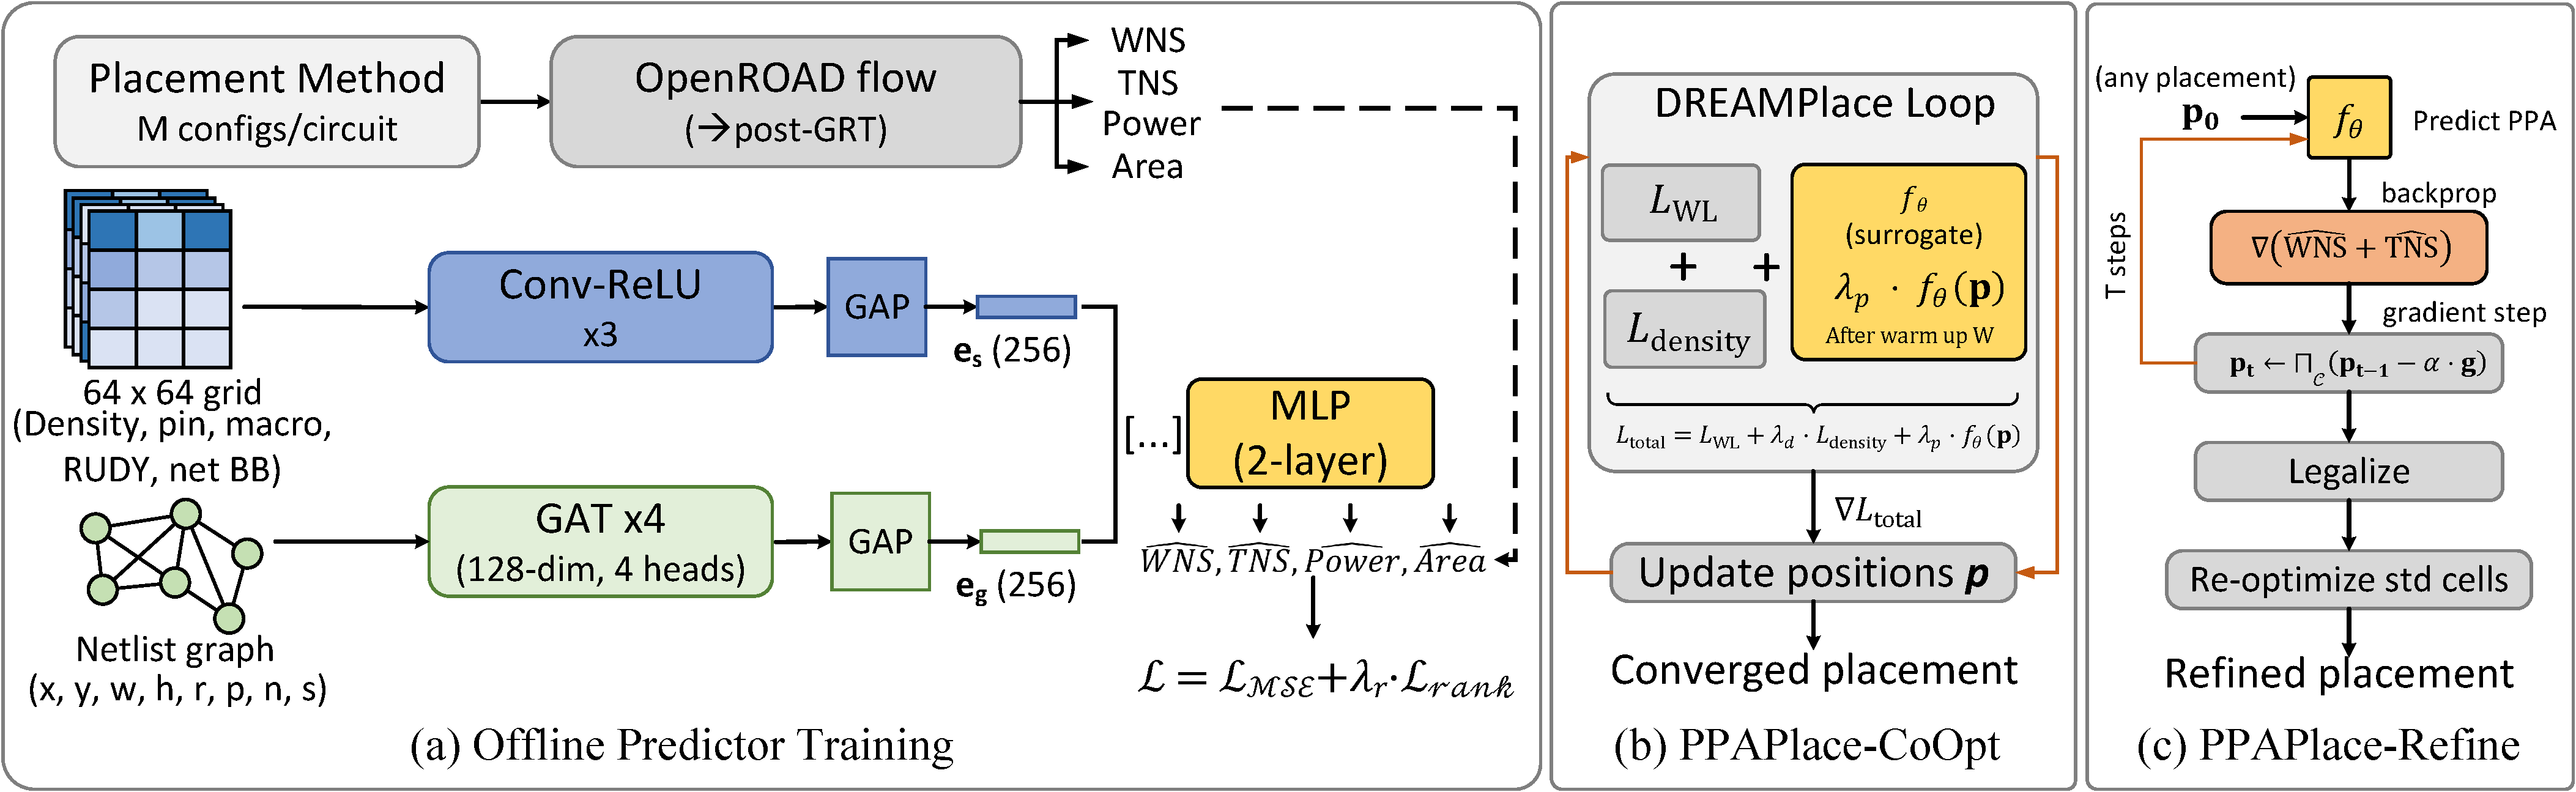
\includegraphics[width=\textwidth]{graphs/ppaplace_overview.pdf}
    \caption{PPAPlace framework.
    (a)~Offline training on post GRT labels.
    (b)~CoOpt injects surrogate gradients into DREAMPlace as a co-objective.
    (c)~Refine applies post placement gradient descent to the converged result.}
    \label{fig:overview}
\end{figure*}

\subsection{Setup}

This study spans 10 ChiPBench~\cite{chipbench2025} circuits. The set
contains RISC-V CPUs from BlackParrot, SweRV, and Ariane, one OpenRISC
CPU, one neural processing unit, and three peripheral designs. Macro
counts range from 10 to 132 and cell counts range from 33K to 427K.
The fidelity study is independent of the training and test split used
for the deployment experiments in Section~\ref{sec:experiments}.

To generate a controlled range of placement qualities, we vary the
weight parameters of OpenROAD's RTLMP hierarchical macro
placer~\cite{ajayi2019openroad}. RTLMP optimizes area utilization,
wirelength, boundary proximity, outline conformance, notch avoidance,
and dead space. For each circuit, we evaluate 20 configurations. The
set contains one default configuration, twelve single parameter sweeps,
and seven multi parameter combinations. This design is a controlled
stratification of the placement quality space. It is not intended to be
a random sample from all possible placements. Because RTLMP is
deterministic for a fixed weight vector, these settings produce 200
unique placements across the 10 circuits.

Each configuration is evaluated through synthesis, floorplanning,
standard cell placement, CTS, GRT, DRT, and timing analysis. WNS, TNS,
and power are recorded at each stage. Area is excluded because it is
fixed by the floorplan within a circuit. The study therefore contains
10 circuits, 20 placements per circuit, and four timing related signals
per placement. Post DRT metrics serve as the ground truth.

\subsection{Stage-Wise Rank Correlation}

Table~\ref{tab:rank_corr} reports Spearman $\rho_{\text{WNS}}$ between
each intermediate signal and post DRT ground truth. HPWL has near zero
average correlation ($\bar\rho = -0.03$), with negative values on 5 of
10 circuits. Pre CTS STA is similarly weak
($\bar\rho = +0.05$). Post CTS is inconsistent. It is strongly positive
on some circuits and negative on others. Post GRT achieves
$\rho \geq 0.78$ on all 10 circuits with no sign reversals
($\bar\rho = 0.86$). It costs $0.20$\,hrs per sample on average versus
$3.7$\,hrs for full DRT.

This pattern agrees with independent observations from
ChiPBench~\cite{chipbench2025}, which reports a Pearson correlation of
$-0.08$ between macro HPWL and WNS, and with LaMPlace~\cite{lamplace2025},
which reports weak HPWL timing correlation under its flow. These
independent results suggest that the HPWL timing gap is not an artifact
of one sweep or one predictor architecture.

\begin{table}[t]
\centering
\caption{Congestion range for held out circuits. Peak RUDY and global route overflow are extracted from placement and OpenROAD reports. The final two columns show HPWL rank correlation with post DRT timing. Placeholder values will be replaced by parsed log values.}
\label{tab:congestion}
\renewcommand{\arraystretch}{1.12}
\footnotesize
\begin{tabular}{@{}l cccc@{}}
\toprule
Circuit & Peak RUDY & GRT overflow & $\rho_{\text{WNS}}$ & $\rho_{\text{TNS}}$ \\
\midrule
swerv\_wrap   & [RUDY_SWERV] & [OVF_SWERV] & [RHO_WNS_SWERV] & [RHO_TNS_SWERV] \\
ariane133     & [RUDY_A133]  & [OVF_A133]  & [RHO_WNS_A133]  & [RHO_TNS_A133] \\
black\_parrot & [RUDY_BP]    & [OVF_BP]    & [RHO_WNS_BP]    & [RHO_TNS_BP] \\
bp\_be        & [RUDY_BPBE]  & [OVF_BPBE]  & [RHO_WNS_BPBE]  & [RHO_TNS_BPBE] \\
ariane136     & [RUDY_A136]  & [OVF_A136]  & [RHO_WNS_A136]  & [RHO_TNS_A136] \\
microwatt     & [RUDY_MICRO] & [OVF_MICRO] & [RHO_WNS_MICRO] & [RHO_TNS_MICRO] \\
jpeg          & [RUDY_JPEG]  & [OVF_JPEG]  & [RHO_WNS_JPEG]  & [RHO_TNS_JPEG] \\
\bottomrule
\end{tabular}
\renewcommand{\arraystretch}{1.0}
\end{table}

Table~\ref{tab:congestion} separates the proxy failure from congestion
coverage. The held out set includes circuits in low, medium, and high
congestion regimes. HPWL remains weakly correlated with final timing
across that range. This supports using post GRT labels as timing
supervision rather than relying on wirelength or pre route STA.


%% ============================================================
\section{PPAPlace}
\label{sec:method}

Based on the findings in Section~\ref{sec:label_fidelity}, PPAPlace
uses post GRT labels as training supervision. PPAPlace has three
components. A differentiable timing surrogate is trained on the mixed
size placement state
(Sections~\ref{subsec:representation} to~\ref{subsec:training}). A
differentiable feature extraction layer enables gradient flow from
predictions back to cell positions
(Section~\ref{subsec:diff_features}). Two gradient-guided deployment
modes, co-objective placement and post-placement refinement, exploit
these gradients to improve post route timing
(Section~\ref{subsec:gradient_placement}).
Figure~\ref{fig:overview} illustrates the overall design.


\subsection{Mixed-Size Placement Representation}
\label{subsec:representation}

Existing cross stage predictors such as LaMPlace~\cite{lamplace2025} represent the
placement state through macro pairwise distances, discarding information
about standard cells, spatial density, and routing congestion. However,
timing violations are largely affected by
standard cell placement and routing, not macro positions
alone~\cite{chipbench2025}. PPAPlace addresses this by observing the
complete mixed size placement through two complementary representations.

\textbf{Spatial representation.} The placement canvas is rasterized into
a $64 \times 64$ grid with five channels:
\begin{enumerate}
    \item Cell density. Total cell area overlapping each bin,
    normalized by bin capacity.
    \item Pin density. Input and output pin concentration per bin.
    \item Macro occupancy. Degree of macro presence in each bin.
    \item RUDY congestion. Estimated routing demand per
    bin~\cite{rudy}, computed as $\sum_{e} 1/(W_e \cdot H_e)$ over
    nets $e$ whose bounding box overlaps the bin, where $W_e$ and $H_e$
    are bounding box dimensions.
    \item Net bounding box density. Net bounding box overlap
    per bin, capturing routing pressure from nets whose
    pins lie outside the bin.
\end{enumerate}
All channels are normalized to $[0, 1]$. This grid-based representation
captures spatial distribution patterns invisible to macro-only
predictors, including congestion hotspots and density imbalances.

\textbf{Graph representation.} The netlist is represented as a graph
$G = (V_G, E_G)$ where macros are the nodes. Edges are derived
from the netlist hypergraph. Each multi-pin net connecting $k$ macros
produces $\binom{k}{2}$ undirected edges (clique expansion), with
duplicate edges merged and edge weights set to the number of shared
nets between each macro pair. Each node carries
a feature vector:
\begin{equation}
\label{eq:node_features}
\mathbf{h}_i = [x_i,\; y_i,\; w_i,\; h_i,\; r_i,\; p_i,\;
n_i,\; s_i],
\end{equation}
where $(x_i, y_i)$ is normalized position, $(w_i, h_i)$ is normalized
width and height, $r_i = w_i / h_i$ is aspect ratio, $p_i$ is pin
count, $n_i$ is net degree (number of nets connected to this node), and
$s_i$ is average net span (mean HPWL of connected nets). 

The two streams are complementary. The spatial grid captures global
density and routing pressure. The graph captures per macro identity and
local connectivity.

\subsection{Dual-Stream Timing Predictor}
\label{subsec:architecture}

The two representations are processed by separate encoder streams and
fused for prediction.

\textbf{Spatial stream.} A lightweight convolutional neural network (CNN) with 3 layers
and ReLU activations progressively reduces the spatial
resolution of the $64 \times 64$ grid. Global average
pooling (GAP) produces
a spatial embedding $\mathbf{e}_s \in \mathbb{R}^{256}$.

\textbf{Graph stream.} A 4-layer graph attention network
(GAT)~\cite{gat2018} with 128-dimensional hidden states and 4
attention heads processes the netlist graph. Multi-head attention allows
each layer to learn different types of relationships between connected
nodes, such as spatial proximity and connectivity strength. GAP aggregates all node embeddings into a fixed-size graph embedding
$\mathbf{e}_g \in \mathbb{R}^{256}$, regardless of circuit size.

\textbf{Fusion and prediction.} The two embeddings are concatenated and
mapped to timing and preservation metrics through a 2-layer multi-layer
perceptron (MLP):
\begin{equation}
\label{eq:predictor}
f_\theta(\mathbf{x}) =
\mathrm{MLP}\!\left([\mathbf{e}_g(\mathbf{x});\;
\mathbf{e}_s(\mathbf{x})]\right) \rightarrow
[\widehat{\mathrm{WNS}},\; \widehat{\mathrm{TNS}},\;
\widehat{\mathrm{Power}},\; \widehat{\mathrm{Area}}].
\end{equation}
The hat notation denotes predicted values. CoOpt and Refine use the WNS
and TNS outputs as the optimization signal. Power and area are retained
for prediction diagnostics, while area is fixed by the floorplan in our
experiments. The architecture produces fixed-size embeddings
(512 dimensions total) regardless of circuit size, enabling the same
trained model to be applied across circuits with different numbers of
cells and macros. Because the pipeline from feature extraction to
prediction is differentiable, the Jacobian
$\partial f_\theta / \partial \mathbf{p}$ is available through automatic
differentiation. This Jacobian indicates how each cell position
influences predicted post route timing.


\subsection{Training}
\label{subsec:training}

\subsubsection{Data Generation}

Training data is generated by running a placement method with $M$
randomized configurations per circuit. Each configuration varies
parameters that affect placement quality, such as target density and
density weight schedule. As discussed in Section~\ref{sec:label_fidelity}, each resulting placement is
evaluated through the OpenROAD flow to post GRT, producing
labels $\mathbf{y}_i = [\mathrm{WNS},\; \mathrm{TNS},\;
\mathrm{Power},\; \mathrm{Area}]$. The training set is
$\mathcal{D} = \{(\mathbf{x}_i, \mathbf{y}_i)\}_{i=1}^{C \times M}$
across $C$ circuits.

\subsubsection{Loss Function}

The predictor is trained with a composite loss:
\begin{equation}
\label{eq:loss}
\mathcal{L} = \mathcal{L}_{\mathrm{MSE}}
+ \lambda_r \cdot \mathcal{L}_{\mathrm{rank}}.
\end{equation}
$\mathcal{L}_{\mathrm{MSE}}$ is the mean squared error between
predicted and true values. However, the core task of the predictor is
not exact metric regression. It is to rank placements by final timing.
Because of this, $\mathcal{L}_{\mathrm{rank}}$ is a pairwise ranking loss
computed over placement pairs from the same circuit:
\begin{equation}
\label{eq:ranking}
\mathcal{L}_{\mathrm{rank}} = \sum_{(i,j)}
\max\!\Big(0,\; -(\mathbf{y}_i - \mathbf{y}_j) \cdot
\big(f_\theta(\mathbf{x}_i) - f_\theta(\mathbf{x}_j)\big)\Big),
\end{equation}
where the sum is over all placement pairs $(i, j)$ from the same
circuit. All four outputs are sign unified (lower is better) and
z-score normalized per circuit. The hinge incurs zero loss for
correctly ranked pairs and a linear penalty for misranked ones,
directly optimizing ordinal accuracy. Power varies by less than 2\%
across configurations of the same circuit, so timing dominates the
ranking signal. With $M = 500$ samples per circuit, each mini-batch
covers $\binom{500}{2} \approx 125$K pairs per epoch.
The MSE term stabilizes learning with an absolute signal, while
the ranking loss optimizes the ordinal accuracy needed for deployment.

\subsection{Differentiable Feature Extraction}
\label{subsec:diff_features}

The feature extraction layer maps cell positions to the spatial grid
and node features of Section~\ref{subsec:representation} through
differentiable operations. This ensures that gradients
$\partial f_\theta / \partial \mathbf{p}$ flow end-to-end from
predicted timing back to cell coordinates. The same differentiable
features are used during both training and gradient-guided placement.

\textbf{Spatial channels.} Each of the five channels is computed as a
continuous function of cell positions. Cell density (channel~0) uses
clamp-based overlap area. This is piecewise linear and differentiable
almost everywhere, matching the functional form DREAMPlace uses for
its density penalty. Pin density (channel~1) uses Gaussian splatting
($\sigma = 1.5$ bin widths), distributing each pin's contribution
smoothly across neighboring bins. Macro occupancy (channel~2) uses
sigmoid soft masks ($\sigma = 20$), producing a near-binary mask with
a smooth transition at macro boundaries. RUDY congestion (channel~3)
computes net bounding boxes via the log-sum-exp smooth approximation
to $\max$ and $\min$ (temperature $\gamma = 10$), matching
DREAMPlace's wirelength smoothing. Net bounding-box density
(channel~4) uses the same Gaussian splatting as channel~1.

\textbf{Node features.} Positions $x_i, y_i$ enter the feature vector
(Eq.~\ref{eq:node_features}) directly. Average net span $s_i$ uses
the same log-sum-exp HPWL approximation as the spatial RUDY channel.
Static features (width, height, pin count, net degree) carry zero
gradient and require no modification. Channel normalization uses
$\mathbf{g}_c / (\max(\mathbf{g}_c) + \epsilon)$, where $\max$ is
differentiable via PyTorch's \texttt{amax}.

The pipeline from cell positions $\mathbf{p}$ through feature
extraction, GAT, CNN, and MLP to predicted timing is differentiable by
construction. The gradient
$\nabla_{\mathbf{p}} f_\theta$ is available via a single backward
pass.


\subsection{Gradient-Guided Placement}
\label{subsec:gradient_placement}

Given the differentiable surrogate $f_\theta$ and a placement \\
$\mathbf{p} = (x_1, y_1, \ldots, x_N, y_N)$, the gradient
$\nabla_{\mathbf{p}} f_\theta$ indicates how each cell's position
affects predicted post route timing. PPAPlace exploits this signal in two
complementary modes.

\textbf{Co-objective placement (PPAPlace-CoOpt).}
The surrogate is injected directly into DREAMPlace's analytical
placement loop as a third objective alongside wirelength and density
(Algorithm~\ref{alg:coopt}). DREAMPlace first runs $W$ warmup
iterations to reach a rough solution within the surrogate's training
distribution. The total objective then becomes:
\begin{equation}
\label{eq:coopt}
\mathcal{L}_{\mathrm{total}} = \mathcal{L}_{\mathrm{WL}}
  + \lambda_d\,\mathcal{L}_{\mathrm{density}}
  + \lambda_p\,(\widehat{\mathrm{WNS}} + \widehat{\mathrm{TNS}}),
\end{equation}
where $\widehat{\mathrm{WNS}}$ and $\widehat{\mathrm{TNS}}$ are the
timing outputs of $f_\theta(\mathbf{p})$ (power and area outputs are
unused, as they are insensitive to placement changes within the same
floorplan), and $\lambda_p$ increases linearly from 0 to its target value over
the remaining iterations. The gradient reaches macros through both
streams and standard cells through the spatial grid's pin-density,
RUDY, and net-bounding-box channels, so CoOpt reshapes standard-cell
clustering as well as macro placement.

\begin{algorithm}[h]
\caption{PPAPlace-CoOpt Co-Objective Placement}
\label{alg:coopt}
\footnotesize
\begin{algorithmic}[1]
\REQUIRE Predictor $f_\theta$, warmup $W$, target weight $\lambda_p^*$,
  total iterations $N$
\STATE Initialize positions $\mathbf{p}_0$ randomly
\FOR{$t = 1, \ldots, N$}
  \STATE $\mathcal{L} \leftarrow \mathcal{L}_{\mathrm{WL}}
    + \lambda_d\,\mathcal{L}_{\mathrm{density}}$
    \hfill\COMMENT{standard DREAMPlace}
  \IF{$t > W$}
    \STATE $\lambda_p \leftarrow \lambda_p^* \cdot (t - W) / (N - W)$
      \hfill\COMMENT{linear ramp}
    \STATE $\mathcal{L} \leftarrow \mathcal{L}
      + \lambda_p\,(\widehat{\mathrm{WNS}} + \widehat{\mathrm{TNS}})$
      \hfill\COMMENT{timing co-objective}
  \ENDIF
  \STATE $\mathbf{p}_t \leftarrow \mathbf{p}_{t-1}
    - \eta\,\nabla_{\mathbf{p}}\mathcal{L}$
    \hfill\COMMENT{GPU-accelerated update}
\ENDFOR
\STATE \textbf{return} placement $\mathbf{p}_N$
\end{algorithmic}
\end{algorithm}

\textbf{Post-placement refinement (PPAPlace-Refine).}
Starting from any converged placement $\mathbf{p}_0$, projected
gradient descent minimizes the surrogate timing objective
(Algorithm~\ref{alg:refine}):
\begin{equation}
\label{eq:refine}
\mathbf{p}_{t+1} = \Pi_\mathcal{C}\!\left(\mathbf{p}_t
  - \alpha\,\nabla_{\mathbf{p}}
  \big[\widehat{\mathrm{WNS}} + \widehat{\mathrm{TNS}}\big]\right),
\end{equation}
where $\alpha$ is the learning rate and $\Pi_\mathcal{C}$ clips to
the die bounding box. The refined macros are then legalized to resolve overlaps and enforce
boundary constraints, and standard cells are re-optimized
with macros fixed. Only the refined macro locations survive this
handoff, so Refine is effectively a macro-position method, whereas
CoOpt reshapes the full mixed-size placement.

The two modes serve different roles. CoOpt reshapes the global cell
topology during placement but requires integration with a specific
analytical placer. Refine adjusts positions locally after placement.
It accepts any legal DEF placement as input, including placements from
tools whose internals are inaccessible. Its accuracy still depends on
how close the input placement distribution is to the training data, as
shown in Section~\ref{subsec:generalization}.

\begin{algorithm}[h]
\caption{PPAPlace-Refine Post-Placement Refinement}
\label{alg:refine}
\footnotesize
\begin{algorithmic}[1]
\REQUIRE Converged placement $\mathbf{p}_0$, predictor $f_\theta$,
  learning rate $\alpha$, steps $T$
\FOR{$t = 1, \ldots, T$}
  \STATE Compute differentiable features from $\mathbf{p}_{t-1}$
  \STATE $\hat{\mathbf{y}} \leftarrow f_\theta(\text{features})$
  \hfill\COMMENT{surrogate prediction ($<$0.1\,s)}
  \STATE $\mathbf{g} \leftarrow \nabla_{\mathbf{p}}
    (\widehat{\mathrm{WNS}} + \widehat{\mathrm{TNS}})$
  \hfill\COMMENT{backprop}
  \STATE $\mathbf{p}_t \leftarrow \Pi_\mathcal{C}(\mathbf{p}_{t-1}
    - \alpha\,\mathbf{g})$
  \hfill\COMMENT{projected gradient step}
\ENDFOR
\STATE Legalize $\mathbf{p}_T$ and re-optimize standard cells
\STATE \textbf{return} refined placement $\mathbf{p}_T$
\end{algorithmic}
\end{algorithm}




%% ============================================================
\section{Experiments and Results}
\label{sec:experiments}

\subsection{Setup}
\label{subsec:setup}

\subsubsection{Benchmarks}
Experiments use ChiPBench~\cite{chipbench2025} circuits with the
Nangate45 library. Ten circuits serve as training data (bp\_fe,
bp\_be12, isa\_npu, bp\_multi, or1200, swerv\_wrapper43, vga\_lcd,
ethernet, dft68, mor1kx). The held out set is reported by lineage.
Group A contains held out circuits with same family relatives in
training, namely swerv\_wrapper, black\_parrot, and bp\_be. Group B
contains unseen family Ariane circuits, namely ariane133 and ariane136.
Group C contains out of domain designs from outside the original
ChiPBench split, namely microwatt and jpeg. If the optional aes design
is used for training diversity, it is excluded from Group C evaluation.
All placements are evaluated through OpenROAD to detailed routing,
yielding WNS, TNS, power, DRC count, and routed wirelength.

\subsubsection{Training}
Per training circuit, 1{,}000 DREAMPlace configurations are sampled
by randomizing 10 hyperparameters: target density
$\in [0.70, 0.90]$, density weight $\in [10^{-5}, 10^{-3}]$
(log-uniform), learning rate $\in [10^{-3}, 0.032]$ (log-uniform),
gamma $\in [2, 10]$, stop overflow
$\in \{0.05, 0.07, 0.10, 0.15\}$, wirelength model \\
$\in \{\text{weighted-average}, \text{log-sum-exp}\}$, global-placement iterations
$\in \{800, 1000, 1200, 1500\}$, macro halo $\in [0, 10]$ sites,
noise ratio $\in [0.01, 0.05]$, and random seed $\in [1, 10^5]$.
Roughly 65\% of sampled configurations yield valid placements
(DREAMPlace convergence and successful OpenROAD flow). The
first 500 successful placements per circuit are retained and
evaluated through the OpenROAD flow to post GRT, producing 5{,}000
training pairs across ten circuits.

The surrogate is trained end to end on these pairs using the composite
loss from Eq.~\ref{eq:loss} with ranking loss weight
$\lambda_r = 0.5$. Within each mini-batch of 32 samples, placements
are grouped by circuit so that ranking pairs compare designs with the
same netlist. The Adam optimizer runs for 200 epochs with learning
rate $5 \times 10^{-4}$ and weight decay $10^{-5}$. All results
report mean $\pm$ std over 3 independent runs with different seeds.

The label fidelity study (Section~\ref{sec:label_fidelity}) uses
RTLMP placements, while training uses DREAMPlace placements. This
does not create a mismatch. The fidelity analysis concerns the
relationship between flow stages and timing metrics, which is a property
of the design flow rather than any specific placer.
Section~\ref{subsec:generalization} validates this empirically.

\subsubsection{Baselines and methods}
Seven baselines represent the current landscape.
Hier-RTLMP~\cite{hierrtlmp2023} is OpenROAD's hierarchical macro
placer and serves as the ChiPBench reference (all metrics normalized
to 1.00). DREAMPlace~\cite{lin2019dreamplace} is the GPU-accelerated
analytical placer run with the default wirelength-and-density
configuration adopted by ChiPBench~\cite{chipbench2025}.
DREAMPlace\,4.0~\cite{dreamplace4} adds pre route STA net weighting
via OpenTimer. We run the authors' open source release with default parameters.
AutoDMP~\cite{autodmp2023} automates DREAMPlace hyperparameter tuning
via multi-objective Bayesian optimization.
MaskRegulate~\cite{maskregulate2024} refines macro placements using RL
with a regularity-based reward.
LaMPlace~\cite{lamplace2025} trains a cross stage predictor on
pre route STA labels and searches with WireMask-EA evolutionary
optimization.
Re$^2$MaP~\cite{re2map2025} uses recursive mixed-size prototyping
with hand engineered cost terms.
LaMPlace results are from its published evaluation
(marked~$^\dagger$). DREAMPlace, AutoDMP, and MaskRegulate results
are from ChiPBench's end-to-end evaluation~\cite{chipbench2025}
(marked~$^\ddagger$). Re$^2$MaP ratios are computed from its
published results under the same OpenROAD flow (marked~$^\S$).

Three PPAPlace configurations are evaluated, all using the same
trained surrogate. PPAPlace-Refine (Algorithm~\ref{alg:refine})
applies $T{=}30$ projected gradient descent steps
($\alpha{=}0.001$) on predicted WNS$+$TNS to a DREAMPlace default
placement, followed by legalization and standard cell re-optimization.
PPAPlace-CoOpt (Algorithm~\ref{alg:coopt}) injects the surrogate as a
co-objective into DREAMPlace's analytical loop. After $W{=}200$ warmup
iterations, the timing loss weight $\lambda_p$ ramps linearly to $0.01$.
PPAPlace-CoOpt{+}Refine applies Refine after CoOpt, combining global
topology guidance with local gradient refinement.

\subsubsection{Hardware and offline cost}
All experiments run on a single NVIDIA RTX A6000 GPU (48\,GB) with an
Intel Xeon Gold 5218R CPU and 64\,GB RAM. DREAMPlace runs on GPU
(${\sim}$24\,s per configuration). Post GRT evaluation runs on CPU
with 16 concurrent OpenROAD processes
($0.2$\,h per sample on average, ranging from ${\sim}0.05$\,h on the
smallest circuits to ${\sim}0.3$\,h on the largest. See
Table~\ref{tab:rank_corr}). Generating all 5{,}000 training labels
takes ${\sim}$63\,h wall-clock with placement and evaluation
pipelined. Model training takes ${\sim}$45\,min. This offline cost is
amortized: the same dataset and model serve all downstream experiments
without additional labeling.


\subsection{Main Results}
\label{subsec:main_results}

\begin{table*}[t]
\centering
\caption{Post route timing and routability of PPAPlace-CoOpt{+}Refine normalized by Hier-RTLMP. Lower WNS, TNS, power, and routed wirelength are better. DRC reports final detailed route violations. Group C values are placeholders until the out of domain flow runs complete.}
\label{tab:main}
\footnotesize
\setlength{\tabcolsep}{5pt}
\resizebox{\textwidth}{!}{%
\begin{tabular}{@{}lllccccc@{}}
\toprule
Group & Circuit & Method & WNS & TNS & Power & DRC & Routed WL \\
\midrule
Same family & swerv\_wrap   & PPAPlace & 0.76\tpm.03 & 0.59\tpm.04 & [PWR_SWERV] & [DRC_SWERV] & [RWL_SWERV] \\
Same family & black\_parrot & PPAPlace & 0.81\tpm.02 & 0.15\tpm.04 & [PWR_BP]    & [DRC_BP]    & [RWL_BP] \\
Same family & bp\_be        & PPAPlace & 0.65\tpm.02 & 0.48\tpm.05 & [PWR_BPBE]  & [DRC_BPBE]  & [RWL_BPBE] \\
\cmidrule(lr){1-8}
Same family & Average       & PPAPlace & 0.74         & 0.41         & [PWR_A]     & [DRC_A]     & [RWL_A] \\
\midrule
Unseen family & ariane133 & PPAPlace & 0.85\tpm.04 & 0.42\tpm.03 & [PWR_A133] & [DRC_A133] & [RWL_A133] \\
Unseen family & ariane136 & PPAPlace & 0.84\tpm.03 & 0.82\tpm.04 & [PWR_A136] & [DRC_A136] & [RWL_A136] \\
\cmidrule(lr){1-8}
Unseen family & Average   & PPAPlace & 0.85         & 0.62         & [PWR_B]    & [DRC_B]    & [RWL_B] \\
\midrule
Out of domain & microwatt & PPAPlace & [G_C1_WNS]   & [G_C1_TNS]   & [PWR_MICRO] & [DRC_MICRO] & [RWL_MICRO] \\
Out of domain & jpeg      & PPAPlace & [G_C2_WNS]   & [G_C2_TNS]   & [PWR_JPEG]  & [DRC_JPEG]  & [RWL_JPEG] \\
\cmidrule(lr){1-8}
Out of domain & Average   & PPAPlace & [GROUP_C_AVG_WNS] & [GROUP_C_AVG_TNS] & [PWR_C] & [DRC_C] & [RWL_C] \\
\midrule
All groups    & Average   & PPAPlace & [ALL_WNS_RATIO] & [ALL_TNS_RATIO] & [ALL_POWER] & [ALL_DRC] & [ALL_RWL] \\
\bottomrule
\end{tabular}}
\end{table*}

\begin{table}[t]
\centering
\caption{Lineage stratified summary of PPAPlace-CoOpt{+}Refine. Ratios are normalized by Hier-RTLMP. Improvements are computed as $1-\text{ratio}$.}
\label{tab:lineage}
\renewcommand{\arraystretch}{1.12}
\footnotesize
\begin{tabular}{@{}lcccc@{}}
\toprule
Group & WNS ratio & TNS ratio & WNS imp. & TNS imp. \\
\midrule
Same family & 0.74 & 0.41 & 26\% & 59\% \\
Unseen family & 0.85 & 0.62 & 15\% & 38\% \\
Out of domain & [GROUP_C_AVG_WNS] & [GROUP_C_AVG_TNS] & [GROUP_C_WNS_IMP]\% & [GROUP_C_TNS_IMP]\% \\
All groups & [ALL_WNS_RATIO] & [ALL_TNS_RATIO] & [AVG_WNS_IMP]\% & [AVG_TNS_IMP]\% \\
\bottomrule
\end{tabular}
\renewcommand{\arraystretch}{1.0}
\end{table}

Table~\ref{tab:main} reports post route timing and routability for the
combined CoOpt{+}Refine flow. Table~\ref{tab:lineage} aggregates the
same results by design lineage. The same family group gives the largest
gain, with WNS and TNS ratios of 0.74 and 0.41. The unseen family Ariane
group remains positive, with WNS and TNS ratios of 0.85 and 0.62. The
out of domain rows provide the final location for microwatt and jpeg
results once those flow runs complete.

The stratified view makes the generalization claim precise. PPAPlace is
strongest when the test placement distribution is close to training.
It remains useful on unseen family designs, but the gain is smaller.
This is the expected behavior of a learned timing model and motivates
the cross placer and out of domain analysis in Section~\ref{subsec:generalization}.

\begin{figure}[h]
    \centering
    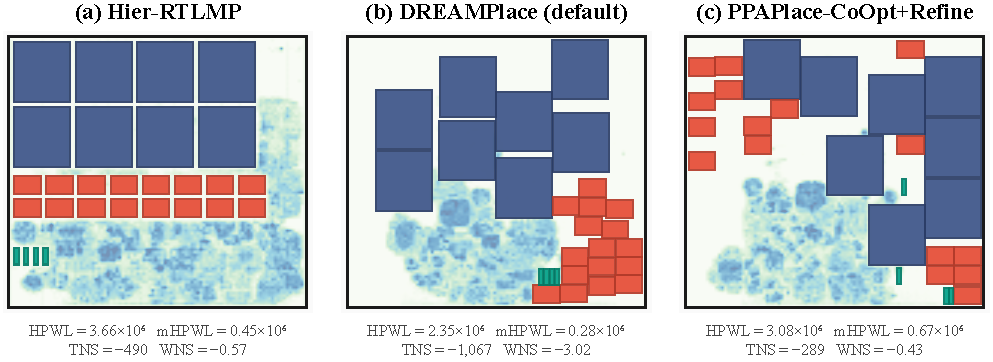
\includegraphics[width=\columnwidth]{graphs/placement_comparison.pdf}
    \caption{Placement comparison on \texttt{swerv\_wrapper}.
    (a)~Hier-RTLMP, (b)~DREAMPlace, (c)~PPAPlace-CoOpt{+}Refine.}
    \label{fig:placement}
\end{figure}

Figure~\ref{fig:placement} illustrates the timing and wirelength tradeoff
on \texttt{swerv\_wrapper}. DREAMPlace reduces HPWL but produces worse
WNS and TNS. PPAPlace-CoOpt{+}Refine accepts a different macro topology
and improves final timing after detailed routing. This matches the label
fidelity result. The learned objective is not a shorter wirelength
objective. It is a timing objective trained from a later flow stage.

Refine alone improves placements when the starting topology is already
near a useful region. It can also fail when the starting placement is far
from the training distribution, as seen on ariane133. CoOpt reduces this
risk by introducing the surrogate after warmup and allowing global
placement topology to adapt before Refine is applied. The combined mode
therefore gives the reported result in Table~\ref{tab:main}.

All values in Table~\ref{tab:main} are final post DRT metrics. The
surrogate is trained on post GRT labels, yet the timing improvements
carry through detailed routing. This is consistent with
Table~\ref{tab:rank_corr}, where post GRT rankings preserve post DRT
timing outcomes with $\bar{\rho}=0.86$.

\begin{figure}[h]
    \centering
    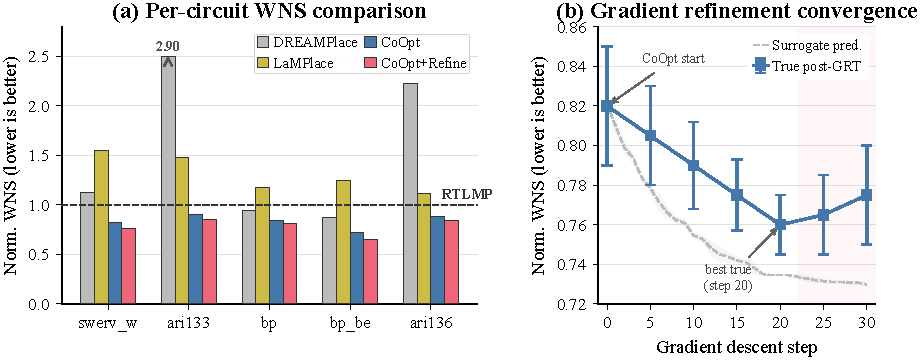
\includegraphics[width=\columnwidth]{graphs/results_main.pdf}
    \caption{(a)~Per-circuit normalized WNS from Table~\ref{tab:main}.
    (b)~True vs.\ surrogate WNS during gradient refinement on swerv\_wrapper.}
    \label{fig:main}
\end{figure}

\subsection{Gradient Quality}
\label{subsec:gradient_quality}

Gradient-guided placement requires directionally accurate gradients.
\texttt{torch.autograd.gradcheck} confirms numerical correctness
(relative error $< 10^{-6}$) on 30 test placements. To assess
directional alignment, we perturb converged placements along 100
random directions per circuit and measure true timing change via
post GRT. Table~\ref{tab:gradient_quality} reports cosine similarity
between surrogate and true gradients: average $0.53$ for WNS and
$0.46$ for TNS, positive on all circuits.

\begin{table}[h]
\centering
\caption{Cosine similarity between surrogate gradient and true post GRT timing change over 100 perturbation directions per circuit.}
\label{tab:gradient_quality}
\renewcommand{\arraystretch}{1.15}
\footnotesize
\begin{tabular}{@{}l cc@{}}
\toprule
Circuit & cos($\nabla$\,WNS) & cos($\nabla$\,TNS) \\
\midrule
swerv\_wrap   & 0.49 & 0.43 \\
ariane133     & 0.58 & 0.49 \\
black\_parrot & 0.51 & 0.46 \\
bp\_be        & 0.62 & 0.53 \\
ariane136     & 0.43 & 0.37 \\
\midrule
Average       & 0.53 & 0.46 \\
\bottomrule
\end{tabular}
\renewcommand{\arraystretch}{1.0}
\end{table}

Figure~\ref{fig:main}(b) validates this on swerv\_wrapper. Gradient
descent reduces true post GRT WNS from $0.82$ to $0.76$ over 20
steps, closely tracked by the surrogate. Beyond step~22, true WNS
rises as the placement exits the training distribution. The
refinement loop retains the best-loss checkpoint across all $T$
steps, so moderate overshoot does not degrade the final result.

We sweep $\lambda_p \in \{0.001, 0.005, 0.01, 0.05\}$ on
swerv\_wrapper, yielding WNS of $\{0.92, 0.87, 0.82, 0.90\}$.
$\lambda_p = 0.01$ provides the best trade-off and is reused
unchanged across all test circuits.
For refinement steps, $T \in \{10, 20, 30, 50\}$ gives WNS
$\{0.79, 0.77, 0.76, 0.77\}$, plateauing at $T{=}30$ before
out-of-distribution degradation begins (Figure~\ref{fig:main}(b)).
The learning rate $\alpha{=}0.001$ is selected by grid search.

\subsection{Generalization}
\label{subsec:generalization}

Table~\ref{tab:generalization} reports ranking accuracy on 500
held out DREAMPlace placements per test circuit. Average Spearman
$\rho = 0.77$ and Kendall $\tau = 0.58$ for WNS, with top-5 accuracy
of 68\% (vs.\ 2\% for random selection). Accuracy is highest on
bp\_be ($\rho = 0.83$) and lowest on ariane136 ($\rho = 0.72$).
Three test circuits share lineage with training circuits
(bp\_be/bp\_be12, swerv\_wrapper/swerv\_wrapper43, black\_parrot/bp\_fe),
which can raise their accuracy. The Ariane circuits have no
training set relatives and show the lowest $\rho$.

\begin{table}[h]
\centering
\caption{Surrogate generalization on held out placements and direct transfer to RTLMP placements.}
\label{tab:generalization}
\renewcommand{\arraystretch}{1.15}
\footnotesize
\begin{tabular}{@{}l ccc cc@{}}
\toprule
& \multicolumn{3}{c}{Held-out (DREAMPlace)}
& \multicolumn{2}{c}{Cross-placer (RTLMP)} \\
\cmidrule(lr){2-4}\cmidrule(lr){5-6}
Circuit & $\rho$ & $\tau$ & Top-5
  & $\rho_\text{WNS}$ & $\rho_\text{TNS}$ \\
\midrule
swerv\_wrap   & 0.74 & 0.56 & 60\% & 0.63 & 0.57 \\
ariane133     & 0.81 & 0.62 & 80\% & 0.58 & 0.54 \\
black\_parrot & 0.77 & 0.55 & 60\% & 0.60 & 0.53 \\
bp\_be        & 0.83 & 0.65 & 80\% & 0.72 & 0.66 \\
ariane136     & 0.72 & 0.51 & 60\% & 0.54 & 0.50 \\
\cmidrule(lr){1-1}\cmidrule(lr){5-6}
bp\_fe\textsuperscript{t}  &  &  &  & 0.68 & 0.60 \\
ethernet\textsuperscript{t}&  &  &  & 0.55 & 0.52 \\
\midrule
Average       & 0.77 & 0.58 & 68\% & 0.61 & 0.56 \\
\bottomrule
\multicolumn{6}{@{}l}{\scriptsize\textsuperscript{t}Training circuit (cross-placer only).}
\end{tabular}
\renewcommand{\arraystretch}{1.0}
\end{table}

\begin{table}[h]
\centering
\caption{Cross placer transfer summary. The mixed source and fine tuning rows are placeholders for the revised experiment.}
\label{tab:cross_placer}
\renewcommand{\arraystretch}{1.12}
\footnotesize
\begin{tabular}{@{}lcc@{}}
\toprule
Training source & $\rho_{\text{WNS}}$ & $\rho_{\text{TNS}}$ \\
\midrule
DREAMPlace only & 0.61 & 0.56 \\
DREAMPlace plus RTLMP mixed source & [MIXED_SOURCE_RHO_WNS] & [MIXED_SOURCE_RHO_TNS] \\
DREAMPlace plus small RTLMP fine tuning & [FINETUNE_RHO_WNS] & [FINETUNE_RHO_TNS] \\
\bottomrule
\end{tabular}
\renewcommand{\arraystretch}{1.0}
\end{table}

Leave-one-circuit-out (LOCO) cross-validation (Figure~\ref{fig:analysis}(a)) trains on
9 circuits and evaluates on the held-out circuit. Per-circuit $\tau$
ranges from $0.07$ (isa\_npu) to $0.28$ (mor1kx), modest individually
but sufficient for the surrogate to consistently identify
above-average placements in deployment.

\begin{figure}[h]
    \centering
    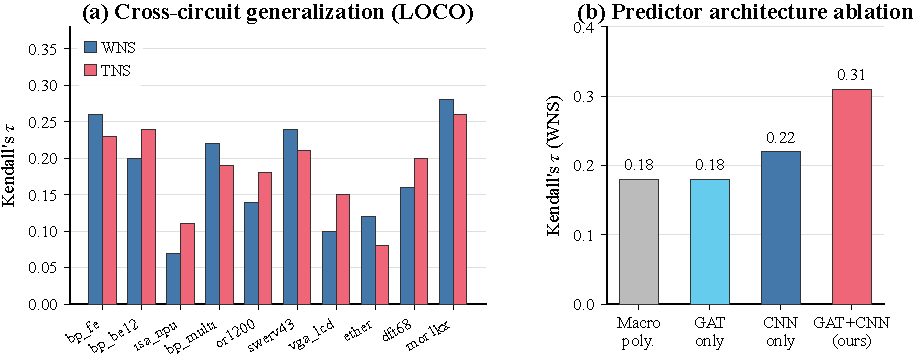
\includegraphics[width=\columnwidth]{graphs/results_analysis.pdf}
    \caption{(a)~Leave-one-circuit-out (LOCO) cross-circuit generalization (Kendall's $\tau$).
    (b)~Predictor architecture ablation (Kendall's $\tau$).}
    \label{fig:analysis}
\end{figure}

Table~\ref{tab:generalization} (right) applies the DREAMPlace-trained
predictor to RTLMP configurations. The predictor has never seen RTLMP
placements during training. Cross-placer $\rho$ averages 0.61 for
WNS, lower than within-placer (0.77) but still positive on all tested
circuits. Table~\ref{tab:cross_placer} gives the location for the
mixed source and small fine tuning experiments. These rows test whether
the transfer gap is mainly a data distribution gap rather than a
limitation of the representation.


\subsection{Ablation Studies}
\label{subsec:ablations}

\begin{table}[t]
\centering
\caption{Ablation on labels and representation using Kendall's $\tau$ for WNS. The upper block is a factorial comparison. The lower block changes only the label stage.}
\label{tab:ablation_combined}
\renewcommand{\arraystretch}{1.15}
\footnotesize
\begin{tabular}{@{}ll cc@{}}
\toprule
Training labels & Architecture & $\tau$ (WNS) & Top-1 \\
\midrule
\multicolumn{4}{@{}l}{\emph{Label and representation}} \\[1pt]
Pre route STA & Macro-only poly.\ & 0.08\tpm.02 & n/a \\
Pre route STA & GAT+CNN & 0.13\tpm.03 & 26\% \\
Post GRT      & Macro-only poly.\ & 0.18\tpm.02 & n/a \\
Post GRT      & GAT+CNN & \textbf{0.31\tpm.02} & \textbf{52\%} \\
\midrule
\multicolumn{4}{@{}l}{\emph{Label stage (GAT+CNN fixed)}} \\[1pt]
Post CTS      & GAT+CNN & 0.16\tpm.03 & 30\% \\
Post DRT      & GAT+CNN & 0.34\tpm.02 & 56\% \\
\bottomrule
\end{tabular}
\renewcommand{\arraystretch}{1.0}
\end{table}

\begin{table}[t]
\centering
\caption{Deployment ablation by supervision stage. Each learned row uses the same GAT+CNN architecture and the same CoOpt{+}Refine deployment. Values report improvement over Hier-RTLMP on the original held out set.}
\label{tab:supervision_deploy}
\renewcommand{\arraystretch}{1.12}
\footnotesize
\begin{tabular}{@{}lcc@{}}
\toprule
Supervision stage & WNS improvement & TNS improvement \\
\midrule
HPWL only DREAMPlace baseline & 0\% & 0\% \\
Pre route STA labels & [PRE_ROUTE_WNS]\% & [PRE_ROUTE_TNS]\% \\
Post CTS labels & [POST_CTS_WNS]\% & [POST_CTS_TNS]\% \\
Post GRT labels & 22\% & 51\% \\
\bottomrule
\end{tabular}
\renewcommand{\arraystretch}{1.0}
\end{table}

\subsubsection{Label Fidelity and Representation}
\label{subsec:2x2}

The upper section of Table~\ref{tab:ablation_combined} crosses two
label stages with two representations under identical training. The macro-only + pre route STA cell ($\tau = 0.08$), which
corresponds to LaMPlace's design choices, is barely above random. Both axes contribute
independently. Post GRT labels double macro-only $\tau$ from 0.08 to
0.18. The GAT+CNN representation raises pre route $\tau$ from 0.08 to
0.13. The combined setting (mixed-size + post GRT) reaches
$\tau = 0.31$.

The lower section isolates the label axis with a fixed GAT+CNN
architecture. Post CTS ($\tau = 0.16$) yields near-random ranking.
Post GRT ($\tau = 0.31$) roughly doubles the correlation. Post DRT
provides a modest further gain ($\tau = 0.34$) at $6\times$ the
labeling cost. Under a fixed 48-hour budget, 500 post GRT samples
($\tau = 0.31$) outperform 80 post DRT samples ($\tau = 0.28$). The
additional data volume from cheaper labels more than compensates for
the slight fidelity gap.

Table~\ref{tab:supervision_deploy} connects the same label choice to
the final placement flow. Replacing post GRT labels with pre route or
post CTS labels leaves little or inconsistent gain. The post GRT row
keeps the same architecture and deployment, which isolates supervision
choice as the main source of the improvement.

\subsubsection{Predictor Architecture}
\label{subsec:pred_results}

The $2 \times 2$ experiment established that the mixed-size
representation matters. Figure~\ref{fig:analysis}(b) unpacks which
components contribute. Four variants are compared, all trained on
post GRT labels. Macro-only polynomial reaches $\tau = 0.18$, CNN-only
($\tau = 0.22$), GAT-only ($\tau = 0.18$), and GAT+CNN
($\tau = 0.31$). The spatial stream alone outperforms the graph
stream alone. Their combination exceeds either single stream,
indicating that density patterns and connectivity structure provide
complementary information.


%% ============================================================
\section{Conclusion}
\label{sec:conclusion}

This paper shows that the supervision stage is a central design choice
for learned placement objectives. HPWL and pre route timing do not
reliably preserve final routed timing rankings. Post GRT does. PPAPlace
uses that observation to train a differentiable timing surrogate over
mixed size placements and then uses its gradients through CoOpt and
Refine. The revised evaluation reports results by design lineage. It
separates same family transfer, unseen family transfer, and out of
domain transfer rather than relying only on a single average.

On the current held out set, CoOpt{+}Refine reduces WNS by 22\% and TNS
by 51\% over Hier-RTLMP. On unseen family Ariane circuits alone, it
reduces WNS by 15\% and TNS by 38\%. The out of domain rows will be
updated with [GROUP_C_WNS_IMP]\% WNS and [GROUP_C_TNS_IMP]\% TNS
improvement after the additional flow runs complete. Across these
settings, power and routability are reported as preservation metrics
rather than as the main optimization target.

\subsection{Limitations}
\label{subsec:limitations}

The current experiments use OpenROAD and the Nangate45 library. Broader
claims across technology nodes, standard cell libraries, and commercial
flows require regenerating the post GRT label corpus in those
environments. The original ChiPBench held out set also contains partial
family overlap with the training set. The stratified results make that
structure explicit. Cross placer transfer remains positive but weaker
than within placer ranking, which indicates a measurable placement
distribution gap. Mixed source training and small target placer fine
tuning are the next experiments for narrowing that gap.

 
%% ============================================================
\newpage
\bibliographystyle{ACM-Reference-Format}
\bibliography{references}

\end{document}
